\chapter{Methodology}\label{ch:methodology}
% \cite{trafton2014blink} 13 ms necessary to recognise objects
This chapter will describe the methodology used to develop the system.
The chapter is divided into five sections.
The first section will describe the data collection process, the second section will describe the data augmentation, the third section will describe the classification model, the fourth section will describe the virtual environment, and the fifth section will describe the evaluation pipeline.
The chapter will conclude with a summary of the methodology used in the development of the system.

\section{Data Collection}
The data collection process is a crucial step in the development of a machine learning system.
It is used to gather the data necessary to train the machine learning model and is divided into two steps: the data collection and the data preprocessing.
The data collection step is used to gather the data necessary to train the machine learning model.
The data preprocessing step is used to clean the data and prepare it for training.
For the first step, we used publicly available EEG motor imagery datasets, such as the BCI Competition IV dataset 2a and the PhysioNet EEG Motor Movement/Imagery Dataset.
These datasets contain EEG recordings of subjects performing motor imagery tasks, such as imagining moving their left or right hand, or their feet.
The datasets contains the preprocessed 64-channel EEG recordings of the subjects, as well as the corresponding labels indicating the class to which the data point belongs.
It is important to notice that we perform some ulterior preprocessing steps, such as filtering and windowing, to clean, split and prepare the data for the training phase.
Also, due to the nature of the dataset recordings, the label distribution is highly unbalanced towards the resting state, so we decided to balance the dataset by undersampling all the data points to the same amount of samples, which was decided to be the lowest class count.
\subsection*{Parameters Used}
To obtain the data, we used the python library MOABB, wich, via the Motor Imagery paradigm, provides simplified access the datasets.
The Motor Imagery paradigm, via its constructor, allows to specify the preprocessing steps.
In this project, we used the following parameters:
\begin{itemize}
    \item \textbf{Channels}: The channels used to record the EEG signals.
    \item \textbf{Events}: The events used to label the data points. In this project, we used the left and right hand, feet and rest motor imagery events.
    \item \textbf{Number of Output Classes}: The number of classes to which the data points belong. In this project, we used 4 classes.
    \item \textbf{Cutoff Frequency for the Bandpass Filter}: The cutoff frequency used to filter the EEG signals. In this project, we used a cutoff frequency of 0.5\textemdash40 Hz.
    \item \textbf{Epoch Start Time}: The time at which the epoch starts. In this project, we used a start time of 0 seconds.
    \item \textbf{Epoch End Time}: The time at which the epoch ends. In this project, we used an end time of 0.5
    \item \textbf{Resampling Frequency}: The frequency at which the data points are resampled. In this project, we used a resampling frequency of 128 Hz.
\end{itemize}
\begin{figure}[!htbp]
    \centering
    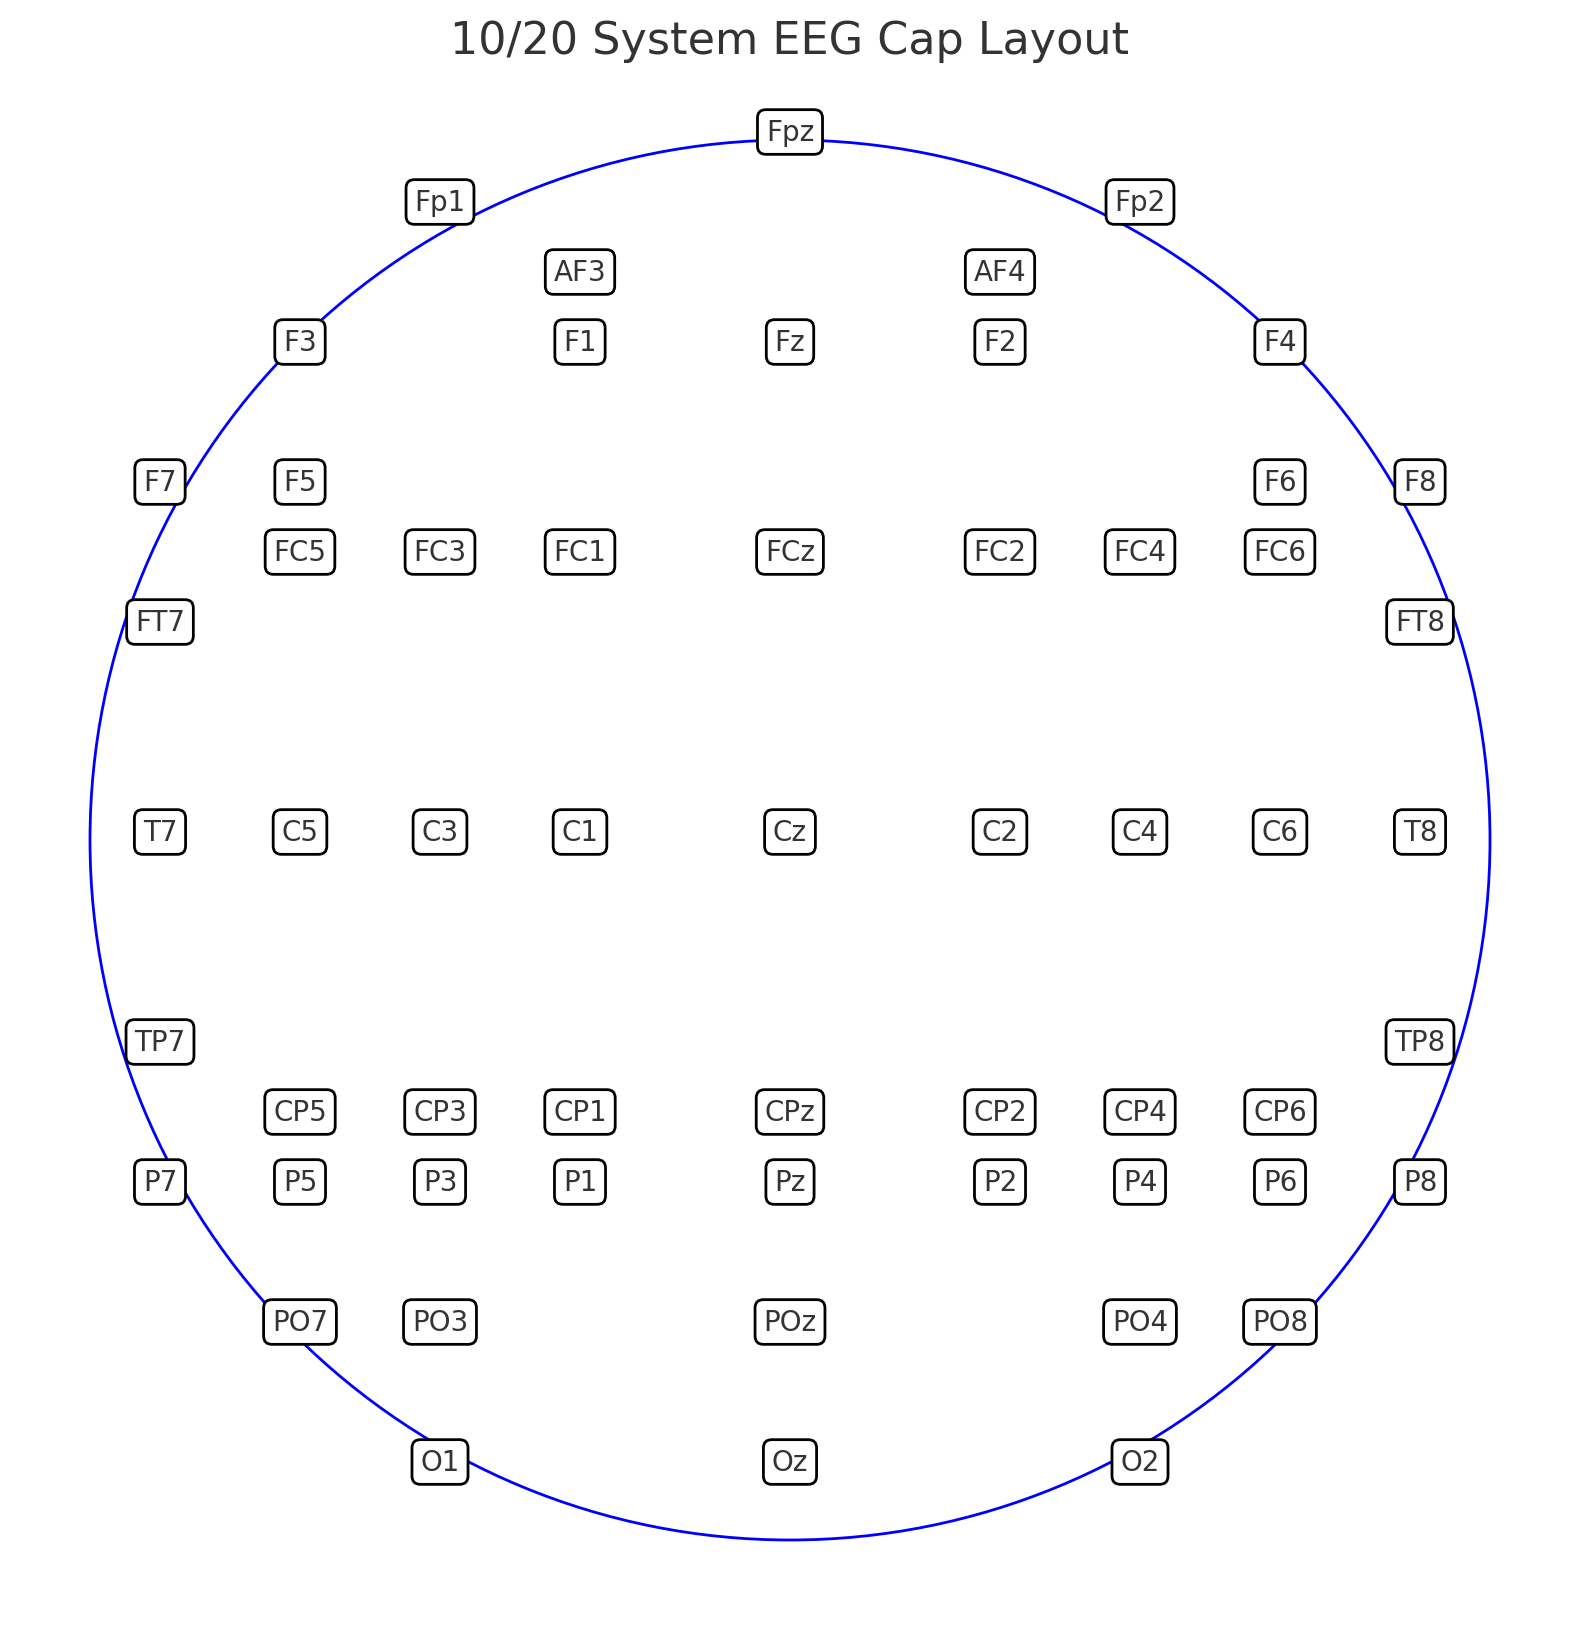
\includegraphics[width=0.5\textwidth]{Figures/Methodology/thesis_eeg_cap}
    \caption{Position of the selected EEG Channels using the reference 10/20 system.}
    \label{fig:eeg_channels}
\end{figure}




\section{Data Augmentation}
Data augmentation is a technique used to increase the size of the training dataset.
It is used to improve the performance of the machine learning model and to generate new data points by applying transformations to the existing ones.
Data augmentation is used to test the generalization of the machine learning model, thus reduce overfitting.
In this project, we applied multiple data augmentation techniques, such as random sampling of the data points, stochastic noise addition, and generation of new data points using GANs.
After testing the quality of the generated data, we found out that the best results were obtained by the noise addition technique and the GAN.

\subsection*{Parameters Used}
For each class, we created a separate genereator, which was used to generate the data points.
Since we are using 4 classes, we created 4 generators using the noise injection and 4 generators using the GAN.
\paragraph*{Stochastic Noise Injection}
The noise injection generator was created by taking the third and fourth quartile of the data points to reduce the size.
After this, we randomly selected a data point from the reduced dataset and added a Gausian noise to it.
The noise was generated using the ``numpy.random.normal'' function, with a mean of 0 and a standard deviation of 1.
As parameter we also provided the shape of the data point, which was used to generate the noise in the correct format.
\paragraph*{Generative Adversarial Networks}
The GAN generator was composed of two networks: the generator (EEGFuseNet) and the discriminator(EFDiscriminator), both network were taken from the models provided by the library ``torcheeg''~\cite{zhang2024torcheeg}.
These models have been reimplemented in torcheeg following their description from~\cite{liang2021eegfusenet}
\begin{figure}[!htbp]
    \centering
    \begin{minipage}[b]{.45\textwidth}
        \centering
        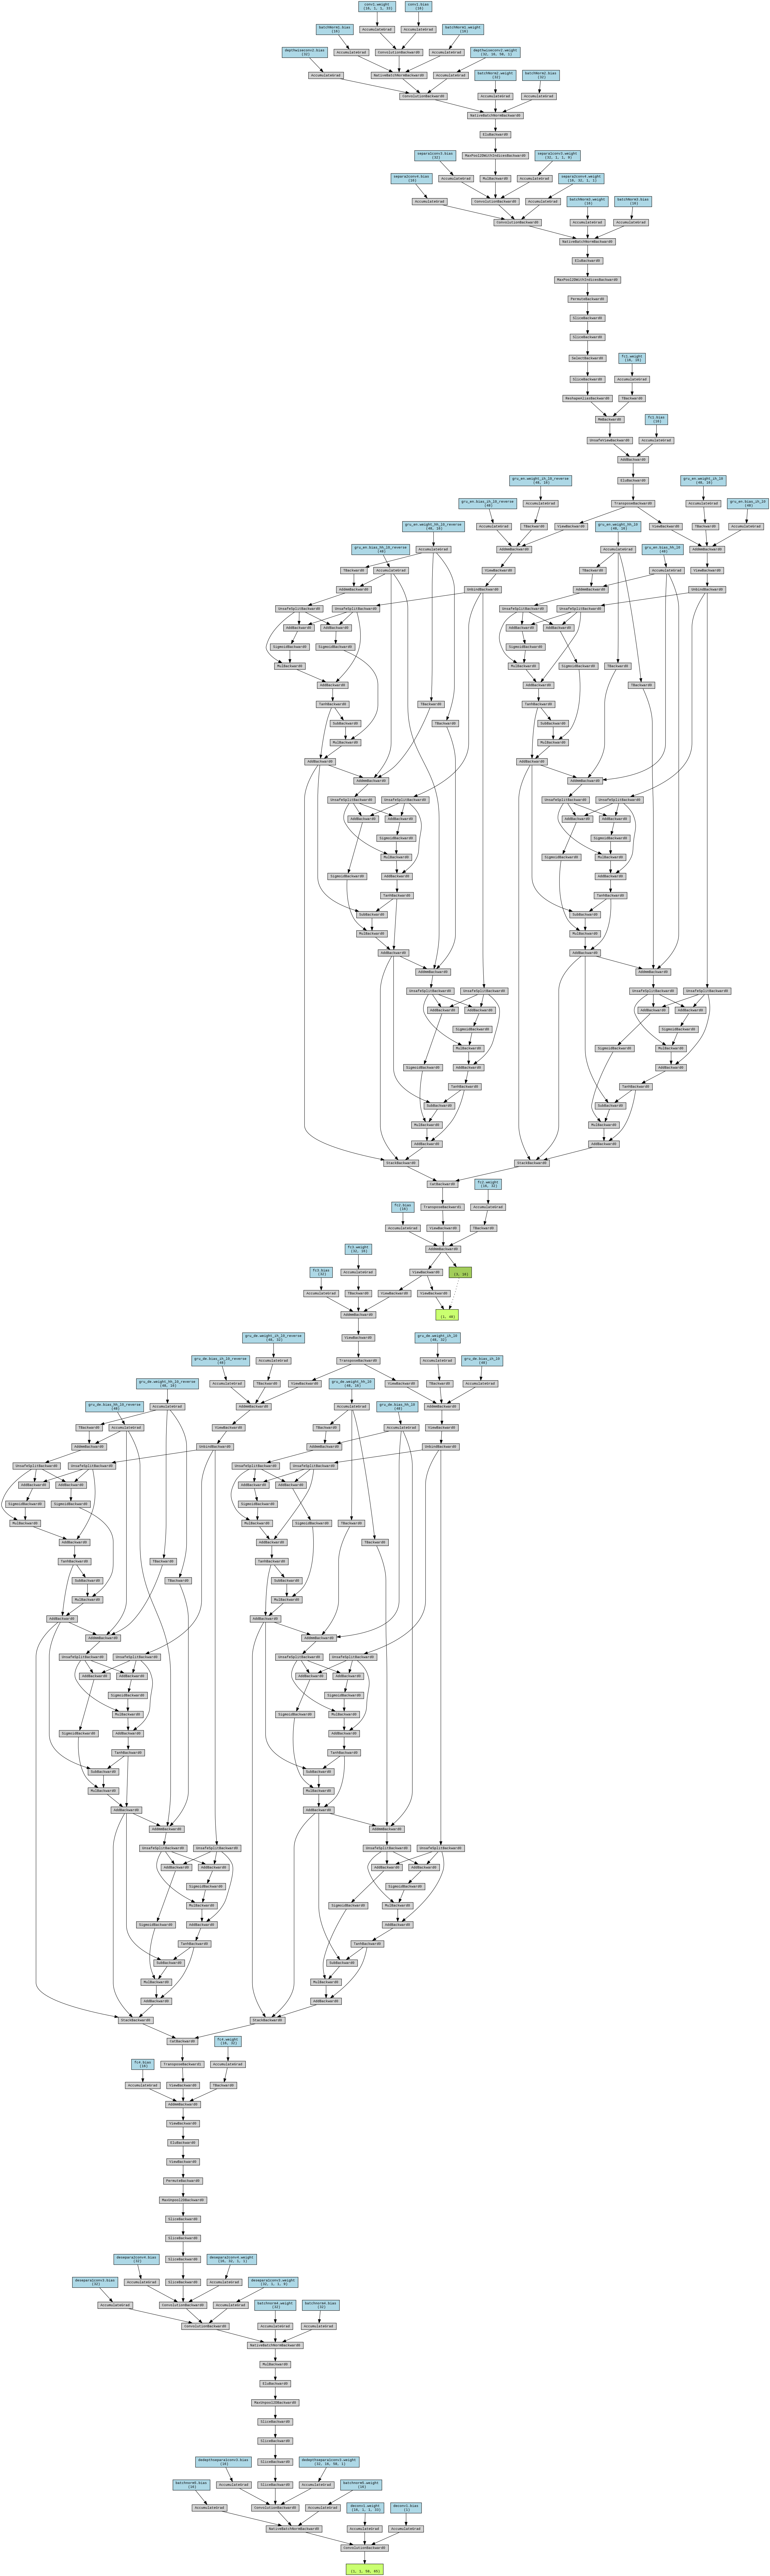
\includegraphics[width=.2\textwidth]{Figures/Methodology/EEGFuseNet}
        \caption{Architecture of the GAN generator.}\label{fig:gan_generator} 
        \vfill   
    \end{minipage}
    \hfill
    \begin{minipage}[b]{.45\textwidth}
        \centering
        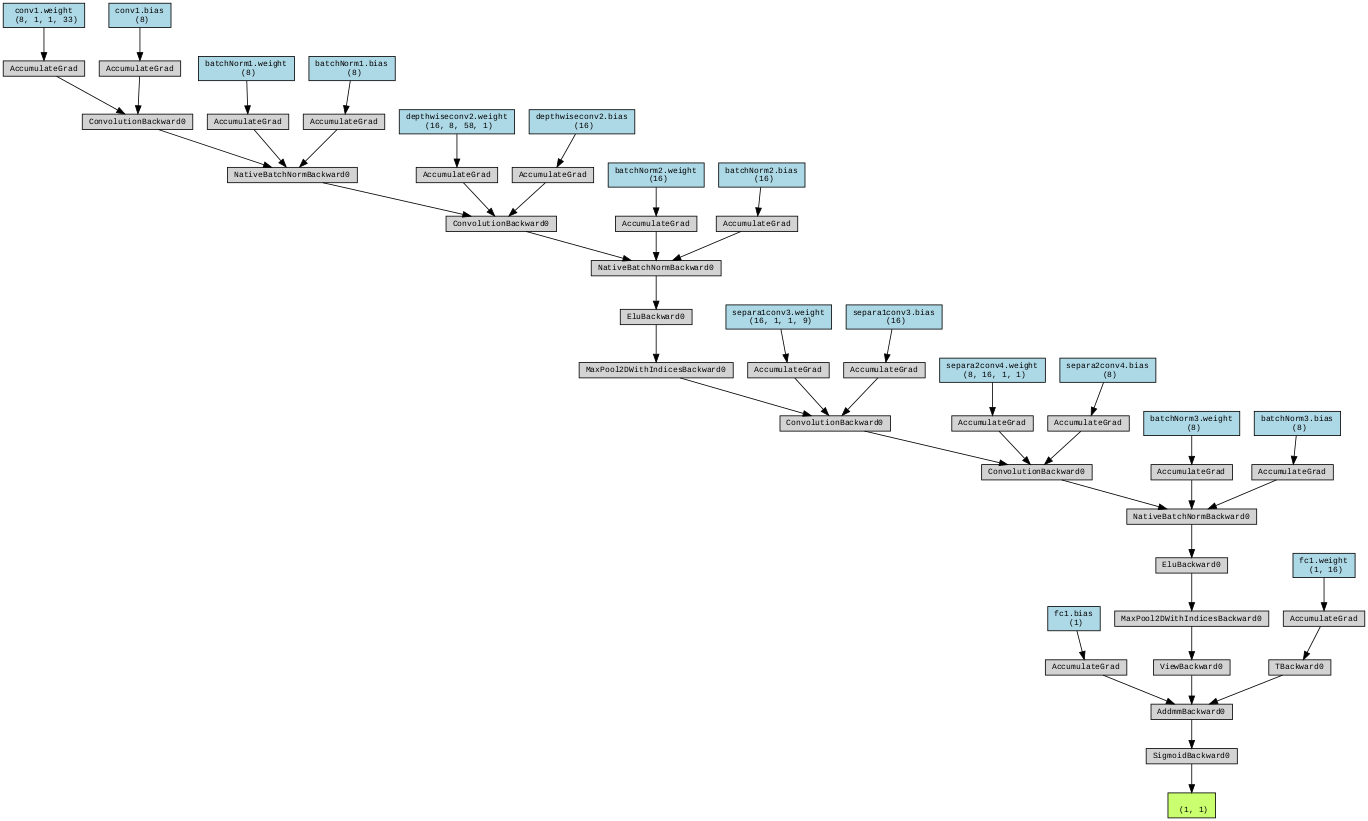
\includegraphics[width=\textwidth]{Figures/Methodology/EFDiscriminator}
        \caption{Architecture of the GAN discriminator.}\label{fig:gan_discriminator}
    \end{minipage}
\end{figure}
\todo{fix the images, replace with simplified ones}


As for the training parameters, we used the following:
\begin{itemize}
    \item \textbf{Loss Function}: Binary Cross Entropy
    \item \textbf{Optimizer}: Adam
    \item \textbf{Learning Rate}: 0.0002
    \item \textbf{Train Epochs}: 100 epochs, each epoch changing the number of steps for generator and discriminator.
\end{itemize}
\paragraph*{Train Epochs}
The training of the GAN was divided into two parts, the generator and the discriminator.
The full training lasted 100 epochs.
During each epoch, we trained the generator and the discriminator for a different number of steps.
The discriminator was trained first, starting with 1000 steps, and decreasing each epoch until 10 steps.
The generator was trained after the discriminator, starting with 10 steps, and increasing each epoch until 1000 steps.


\section{Classification Model}
The classification model is a machine learning or deep learning model used to classify the data points.
It is used to predict the class or label to which the input data point belongs.
In this project, we decided to train a set of machine learning and deep learning models to classify the data points.
Some of these methods, including support vector machines, linear discriminant analysis and convolutional neural networks, have been used as baseline models, the proposed LSTM method has been used as the main model.
We also tried developing an attention based model, but the hardware requirements were too high for the available resources.
The models were trained using the available datasets, and validated using the test set.
Also, the models where evaluated using the generated data points to test their generalization capabilities.
\todo{add the parameters of the model and the figure}

\section{Virtual Environment}
The virtual environment is a computer-generated environment that simulates the real world or a specific scenario.
It is used to test the performance and usability of the machine learning model, and to evaluate the user experience.
In this project, we developed two virtual environments: an infinite runner game where the user can jump over obstacles or move to left or right, and a maze where the user can freely move their character to collect coins.
The virtual environments were developed using the Unity game engine and were designed to be simple and easy to use, and to provide a fun and engaging experience for the user.
The virtual environments were also designed to be controller agnostic, requiring a WebSocket connection to receive the character input commands.

\section{The Framework}
The framework was developed to integrate all the components of the system and to provide a user-friendly interface.
It works as a pipeline that connects the data augmentation or collection from the headset, classification model, and virtual environment.
The framework is plug-and-play, meaning that it can be easily extended to support new data augmentation or generation methods, classification models, virtual environments or real devices.
The framework is also designed to be easy to use, only requiring the paths to the models files and the WebSocket address to send messages.
